\section{Esecuzione}

La prima operazione da noi fatta è stata quella di mettere in moto l'impianto da vuoto portando la camera a una pressione di $10^{-3}$ \si{\pascal}, avendo cura di controllare la pressione raggiunta con il vacuometro a catodo freddo.

In seguito abbiamo misurato l'andamento della pressione interna della camera da vuoto in funzione del tempo con la valvola a spillo completamente chiusa. Ciò è necessario per misurare la variazione della pressione in camera che, una volta isolata dalla pompa turbomolecolare e dal resto dell'impianto, è dovuta ai soli effetti di degasamento.

Una volta eseguita questa prima serie di misure abbiamo riportato la camera ad una pressione interna di $10^{-3}$ \si{\pascal} per misurare il flusso in entrata a seconda dell'apertura della valvola. Abbiamo osservato la seguente procedura:
\begin{itemize}
	\item{portare la camera da vuoto\footnote{La valvola a spillo presenta al suo interno un volume morto di aria a pressione atmosferica, che se ignorato renderebbe scorrette le misure. Per ovviare a questo problema abbiamo chiuso la valvola con un tappo e un O-ring in viton e non con la manopola della stessa, in modo tale da rendere il volume morto parte della camera e quindi avere ovunque la stessa pressione misurata dal vacuometro a catodo freddo.} ad una pressione di circa $10^{-3}$ \si{\pascal}, controllando con il vacuometro a catodo freddo di essere ad una pressione minore del fondoscala del vacuometro Pirani;}
	\item{spegnere il vacuometro a catodo freddo per evitare l'usura o il deterioramento dello stesso a causa dell'aumento di pressione;}
	\item{isolare la camera da vuoto e aprire la valvola a spillo del numero di giri voluto;}
	\item{togliere il tappo posto a chiusura della valvola a spillo e misurare, tramite il multimetro e il sistema di acquisizione dati, il variare della pressione interna della camera in funzione del tempo;}
	\item{infine riportare la camera da vuoto ad una pressione dell'ordine $10^{-3}$ \si{\pascal}, isolando la pompa turbomolecolare e usando quella rotativa qualora necessario;}
\end{itemize}
Mentre la prima serie di misure è stata fatta con la valvola a spillo completamente chiusa, le misure successive hanno invece avuto lo scopo di ottenere i dati di flusso per un'apertura della valvola da 1 a 9 giri completi e di 5.2, 5.4, 5.6 e 5.8 giri.\\

Grazie alle condizioni meteorologiche stabili, l'intera esperienza è stata svolta in laboratorio ad una temperatura ambiente di $294 \pm 0.5$ \si{\kelvin}, una pressione atmosferica di $981 \pm 0.5$ hPa ed una umidità del $55 \pm 0.5$ \%. Le incertezze di queste ultimi dati sono di risoluzione.

\begin{figure}[h!]
    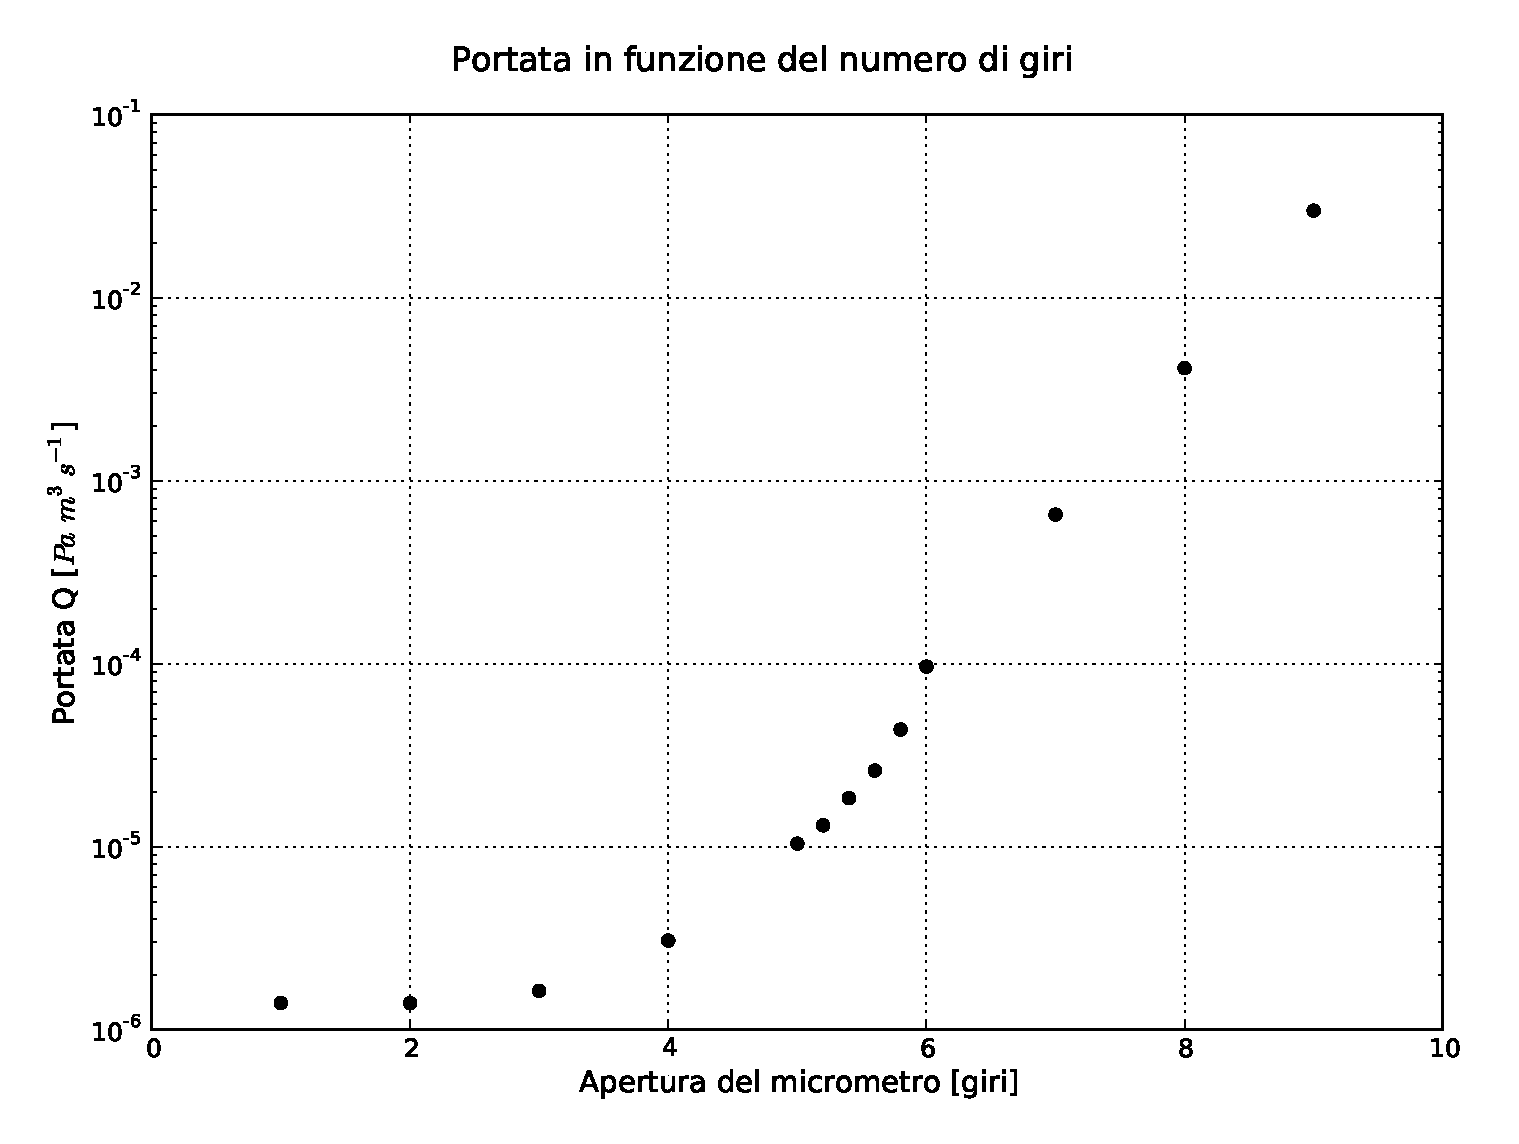
\includegraphics[width=15cm]{graph.pdf}
    \caption{Il grafico mostra i valori elaborati del flusso in entrata a seconda dell'apertura della valvola a spillo. Le barre d'errore non sono
    mostrate in quanto comparabili con la dimensione dei punti sul grafico. L'asse delle ordinate ha scala logaritmica.}
    \label{fig:graph}
\end{figure}

\section{Analisi dati}

Per ogni serie di dati abbiamo ricavato, con il metodo della regressione lineare, un valore della variazione di pressione $\frac{dP}{dt}$. Grazie a questi dati abbiamo poi potuto ottenere una stima del flusso in entrata grazie alla seguente relazione:

\begin{equation}
	Q_{tot} \,\, = \,\, V \frac{dP}{dt}
\end{equation}

Bisogna prestare attenzione che il flusso calcolato ($Q_{tot}$) grazie alla precedente equazione rappresenta il contributo di due differenti fattori: uno è dovuto alla perdita controllata di gas da parte della valvola a spillo ($Q_{valve}$), mentre il secondo è opera degli effetti di degasamento della camera da vuoto e delle altre parti dell'impianto ($Q_{deg}$).

Pertanto, per ricavare Q$_{valve}$ abbiamo dovuto sottrarre al flusso totale calcolato il flusso  dovuto alle perdite intrinseche e virtuali del sistema, ovvero:

\begin{equation}
	Q_{valve} \, = \, Q_{tot} \, - \, Q_{deg} \, = \, V \left[ \frac{dP}{dt} - \left(\frac{dP}{dt}\right)_{deg} \right]
\end{equation}

Dai dati sul flusso $Q_{valve}$ si può ricavare la conduttanza $C$ della valvola:

\begin{equation}
	Q_{valve} \, = \, C (P_{atm} - P) \quad \implies \quad C = \frac{Q_{valve}}{P_{atm} - P} = \frac{Q_{valve}}{P_{atm}}
\end{equation}
%
dove $P$ è la pressione all'interno della camera e $P_{atm}$ è la pressione atmosferica. Nell'ultimo passaggio si è supposto
che $P \ll P_{atm}$, approssimazione vera con buona precisione.

I risultati numerici sono esposti nella tabella sottostante, dove sono riportati i flussi e le conduttanze della valvola ottenute.
Nella prima riga è riportato il flusso di degasamento, e chiaramente non è presente la conduttanza.

\begin{table}
    \begin{tabular}{l c c c c c c}
        \toprule
        Nr. giri &
        $Q  [\si{\Pa\cubic\meter\per\second}]$ & $\sigma (Q) [\si{\Pa\cubic\meter\per\second}]$ &
        $S\ped{rotativa} [\si{\cubic\meter\per\second}]$ & $\sigma (S\ped{rotativa}) [\si{\cubic\meter\per\second}]$ &
        $S\ped{turbo} [\si{\cubic\meter\per\second}]$ & $\sigma (S\ped{turbo}) [\si{\cubic\meter\per\second}]$ \\
        \midrule
        1   & 0.00013 & 1.8617e-06 &                   &                   & 0.029125        & 0.00293821154865 \\
        2   & 0.00013 & 1.962e-06  &                   &                   & 0.02879375      & 0.00290824293227 \\
        3   & 0.00016 & 2.2002e-06 &                   &                   & 0.032572        & 0.00328678977752 \\
        4   & 0.00030 & 2.7229e-06 & 0.000131855016235 & 1.32373703717e-05 & 0.03608         & 0.00362219304695 \\
        5   & 0.00103 & 1.3016e-05 & 0.000315597117771 & 3.18067226996e-05 & 0.0399346153846 & 0.00402471748356 \\
        5.2 & 0.00130 & 8.3042e-06 & 0.000351827594516 & 3.52537345308e-05 & 0.040834375     & 0.00409167512276 \\
        5.4 & 0.00184 & 1.1322e-05 & 0.000413355664841 & 4.14134836725e-05 & 0.0438833333333 & 0.00439660530404 \\
        5.6 & 0.00260 & 1.6312e-05 & 0.000478897721927 & 4.79837415967e-05 & 0.04732         & 0.00474128513959 \\
        5.8 & 0.00436 & 2.6838e-05 & 0.000592110619957 & 5.93229678244e-05 & 0.04848         & 0.00485716246794 \\
        6   & 0.00962 & 0.00012289 & 0.000764887079965 & 7.71090559735e-05 & 0.0458547619048 & 0.00462266587445 \\
        7   & 0.06517 & 0.00055883 & 0.00135131654975  & 0.000135627555918 &  & \\
        8   & 0.41163 & 0.0056583  & 0.00176213082573  & 0.000177870106921 &  & \\
        9   & 2.9884  & 0.067334   & 0.00178338842667  & 0.000182809766946 &  & \\
        \bottomrule
    \end{tabular}
\end{table}













































La tabella ed il relativo grafico in Figura \ref{fig:graph} mostrano chiaramente che l'andamento del flusso non è lineare con
l'apertura della valvola, anzi gli ultimi punti del grafico sembrano suggerire un andamento esponenziale (che su un grafico
con scala logaritmica come quello riportato in figura, risulta in una linea retta). Tuttavia i primi 2/3
punti deviano in maniera vistosa da tale andamento.
